\section{Memory Interface}
\begin{itemize}
  \item Four common types of memory:
  \begin{enumerate}
    \item Read Only Memory (ROM)
    \item Flash memory (EEPROM)
    \item Static Random Access Memory (SRAM)
    \item Dynamic Random Access Memory (DRAM)
  \end{enumerate}

  \item Pin connections common to all memory devices :
  \begin{enumerate}
    \item address inputs
    \item data outputs (inputs/outputs)
    \item some type of selection input
    \item Atleast one control input used to select a read or write operations
  \end{enumerate}
  \item Control connections:
  \begin{enumerate}
    \item \textbf{ROM} $\longrightarrow$ Only one control input ($\overline{OE}$[Output Enable] or $\overline{G}$[Gate])
    \item \textbf{RAM} $\longrightarrow$ Only one($R/\overline{W}$) or two ($\overline{WE}/\overline{W}$ and $\overline{OE}/\overline{G}$) control input. [$\overline{WE}/\overline{W}$ and $\overline{OE}/\overline{G}$ do not get actualed at the same time]
  \end{enumerate}
\end{itemize}

\begin{figure}[h!]
  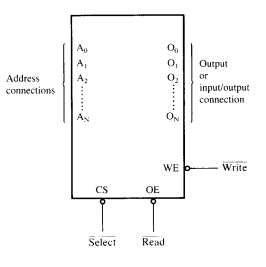
\includegraphics[width = 0.8\textwidth]{./figures/Memory.png}
  \caption{A pseudo-memory component illustrating the address, data, and control connections.}
  \label{}
\end{figure}

\subsection{ROM Memory (nonvolatile memory)}
\begin{itemize}
  \item Permanently stores programs that are resident to the system and must \textbf{not} change when power supply is disconnected (permanently programmed) for example BIOS.
  \item \textbf{EPROM} (Erasable Programmable ROM): Programmed using a device called EPROM programmer; erasable if exposed to high-intensity UV light for about 20 minutes or less.
  \item \textbf{PROM} (Programmable ROM): Programmed by burning open tiny NI-Chrome or Silicon Oxide fuses; Once programmed, it cannot be erased
  \item \textbf{Read Mostly Memory}(RMM) or \textbf{Flash memory} or \textbf{EEPROM}(Electrically Erasable Programmable ROM) or \textbf{EAROM}(Electrically Alterable ROM) or \textbf{NOVRAM}(Non volatile RAM) : Electrically erasable however, needs more time to erase than a normal RAM.
\end{itemize}
\subsection{Delays in operation od an EPROM}
$t_{acc1}$ : Address to output delay\\
$t_{OH}$ : Address to output hold\\
$t_{CO}$ : Chip Select to Output delay\\
$t_{DF}$ : Chip Deselect to Output float\\

\begin{figure}[h!]
  \centering
  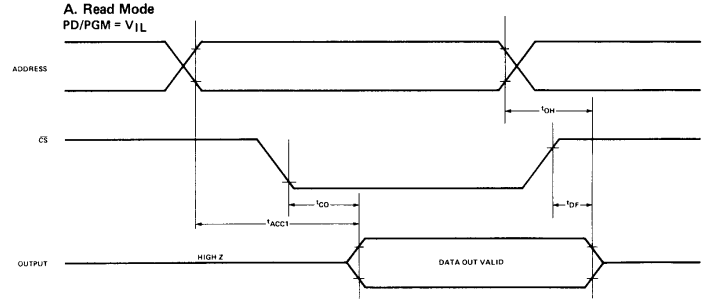
\includegraphics[width = 1.0\textwidth]{./figures/Memory_waveform.png}
  \caption{The timing diagram of AC characteristics of the 2716 EPROM.}
  \label{}
\end{figure}

\subsection{Static memory or static RAM(SRAM) or Volatile memory}
\begin{itemize}
  \item Retain data as long as DC power is applied (no data without power)
  \item Difference between ROM and RAM :
  \begin{itemize}
    \item \textbf{RAM} $\longrightarrow$ written under normal operation
    \item \textbf{ROM} $\longrightarrow$ programmed outside the computer and is normally read.

  \end{itemize}
\end{itemize}


\subsection{Dynamic Ram (DRAM)}
\begin{itemize}
  \item DRAM is essentially same as SRAM, except that it retains data for only 2 or 4ms on an integrated capacitor
  \item After 2 or 4 ms, the contents of DRAM must be completely rewritten (refreshed) because the capacitors (which store Logic 1/0) lose their charges.
  \item Refreshing also occurs during a write, a read, or during a special refresh cycle.
  \item Have much larger sizes compared to SRAM. Its obvious disadvantage is requirement of many address pins. To reduce the number of address pins, the address inputs are multiplexed.
\end{itemize}
\newpage
Example of multiplexed address pins : 64K x 4 DRAM
\begin{figure}[h!]
  \centering
  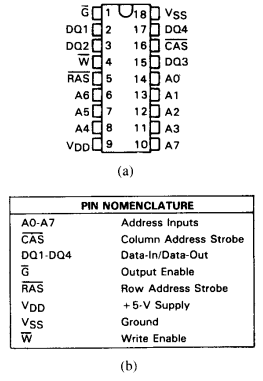
\includegraphics[width = 0.6\textwidth]{./figures/DRAM.png}
  \caption{The pin-out of the TMS4464, 64K x 4 dynamic RAM (DRAM).}
  \label{}
\end{figure}
Here, for 64K, 16 address pins are required. However, 8 address pins are used through multiplexing.
\begin{itemize}
  \item At first, A0 - A7 are stored in internal row latch as row address through enabling $\overline{RAS}$
  \item Next, A8-A5 are stored in internal column latch as column address through enabling $\overline{CAS}$
\end{itemize}
Address multiplexer of 64K x 4

\begin{figure}[h!]
  \centering
  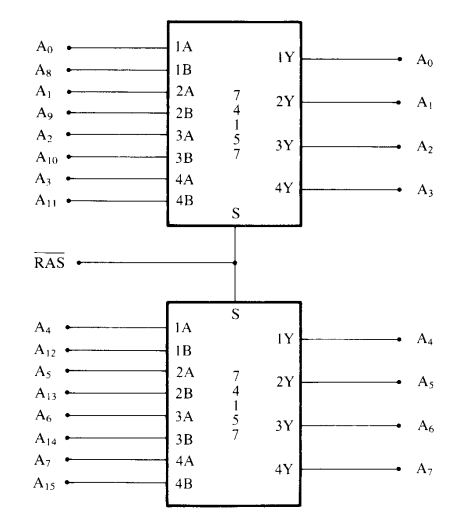
\includegraphics[width = 0.8\textwidth]{./figures/RAS.png}
  \caption{Address multiplexer for the TMS4464 DRAM.}
  \label{}
\end{figure}
\begin{itemize}
  \item If $\overline{RAS}$ is 0, then A pins get connected and A0-A7 are stored in the internal Row Address latch
  \item \textit{Internal Row Address Latch} is edge triggered, and therefore the row address gets captured into the latch before the address changes to column address.
  \item If $\overline{RAS}$ is 1, the the 8 pins get connected and A8-A15 are stored in \textit{Internal Column Address Latch}
\end{itemize}
